% Created 2023-02-16 jue 18:04
% Intended LaTeX compiler: pdflatex
\documentclass[aspectratio=169, usenames,svgnames,dvipsnames]{beamer}
\usepackage[utf8]{inputenc}
\usepackage[T1]{fontenc}
\usepackage{graphicx}
\usepackage{longtable}
\usepackage{wrapfig}
\usepackage{rotating}
\usepackage[normalem]{ulem}
\usepackage{amsmath}
\usepackage{amssymb}
\usepackage{capt-of}
\usepackage{hyperref}
\usepackage{color}
\usepackage{listings}
\usepackage{mathpazo}
\usepackage{gensymb}
\usepackage{amsmath}
\usepackage{diffcoeff}
\usepackage{steinmetz}
\usepackage{mathtools}
\usepackage{fancyvrb}
\DefineVerbatimEnvironment{verbatim}{Verbatim}{fontsize=\tiny, formatcom = {\color{black!70}}}
\bibliographystyle{plain}
\usepackage{siunitx}
\sisetup{output-decimal-marker={,}}
\DeclareSIUnit{\watthour}{Wh}
\DeclareSIUnit{\wattpeak}{Wp}
\DeclareSIUnit{\watthour}{Wh}
\DeclareSIUnit{\amperehour}{Ah}
\usepackage{steinmetz}
\hypersetup{colorlinks=true, linkcolor=Blue, urlcolor=Blue}
\renewcommand{\thefootnote}{\fnsymbol{footnote}}
\parskip=5pt
\usetheme{Boadilla}
\usecolortheme{rose}
\usefonttheme{serif}
\author{\href{https://oscarperpinan.github.io}{Oscar Perpiñán Lamigueiro}}
\date{}
\title{Variabilidad de la Potencia de una Central Fotovoltaica}
\subtitle{Energía Solar Fotovoltaica}
\institute[UPM]{Universidad Politécnica de Madrid}
\setbeamercolor{alerted text}{fg=blue!50!black} \setbeamerfont{alerted text}{series=\bfseries}
\AtBeginSubsection[]{\begin{frame}[plain]\tableofcontents[currentsubsection,sectionstyle=show/hide,subsectionstyle=show/shaded/hide]\end{frame}}
\AtBeginSection[]{\begin{frame}[plain]\tableofcontents[currentsection,hideallsubsections]\end{frame}}
\beamertemplatenavigationsymbolsempty
\setbeamertemplate{footline}[frame number]
\setbeamertemplate{itemize items}[triangle]
\setbeamertemplate{enumerate items}[circle]
\setbeamertemplate{section in toc}[circle]
\setbeamertemplate{subsection in toc}[circle]
\hypersetup{
 pdfauthor={\href{https://oscarperpinan.github.io}{Oscar Perpiñán Lamigueiro}},
 pdftitle={Variabilidad de la Potencia de una Central Fotovoltaica},
 pdfkeywords={},
 pdfsubject={},
 pdfcreator={Emacs 28.2 (Org mode 9.6)}, 
 pdflang={Spanish}}
\begin{document}

\maketitle

\section{Introducción}
\label{sec:org95cdf4a}

\begin{frame}[label={sec:orgfae1d7d}]{Los Sistemas Fotovoltaicos y la Red Eléctrica}
Los sistemas fotovoltaicos conectados a red alteran las condiciones de
funcionamiento habitual de la red.

\begin{center}
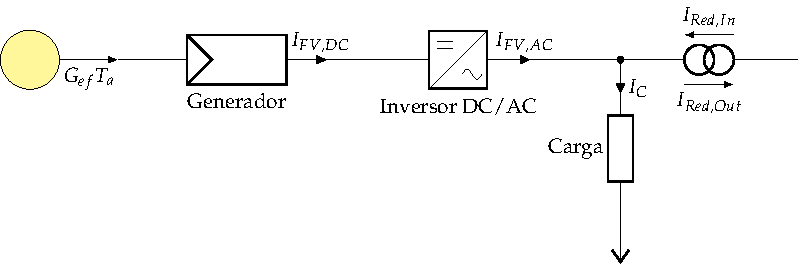
\includegraphics[width=\textwidth]{../figs/SFCR_bidireccional.pdf}
\end{center}
\end{frame}

\begin{frame}[label={sec:org3155ed0}]{Los Sistemas Fotovoltaicos y la Red Eléctrica}
\begin{itemize}
\item Posibilitan la bidireccionalidad del flujo de potencia, con los
consiguientes cambios en la tensión de los nodos, y en la corriente
conducida por las líneas y transformadores.
\end{itemize}

\begin{center}
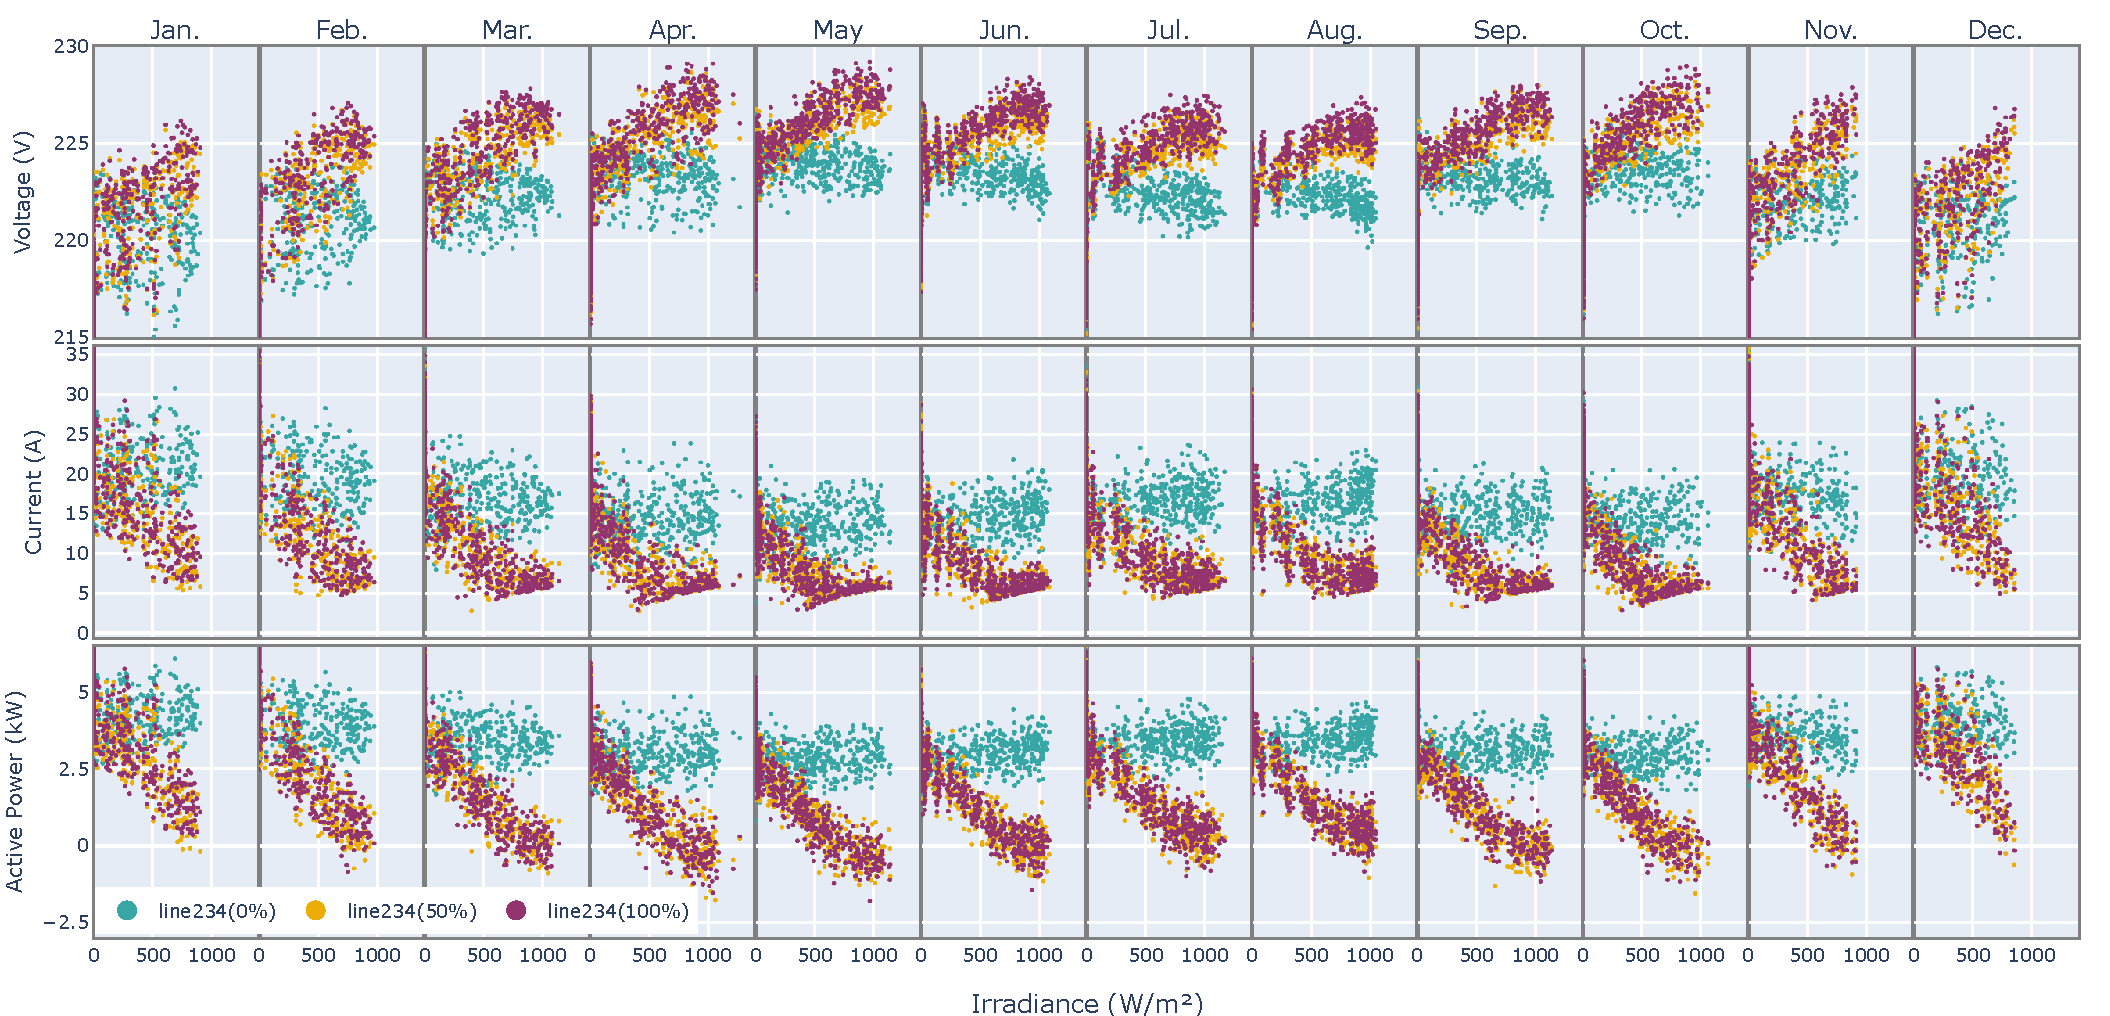
\includegraphics[height=0.7\textheight]{../figs/S_VIP_Irr_line234.pdf}
\end{center}
\end{frame}

\begin{frame}[label={sec:orgf23690a}]{Los Sistemas Fotovoltaicos y la Red Eléctrica}
\begin{itemize}
\item Las rampas de potencia debidas a las fluctuaciones de radiación
solar pueden entorpecer el adecuado funcionamiento de los equipos
conectados a la red y los elementos de protección existentes.

\begin{center}
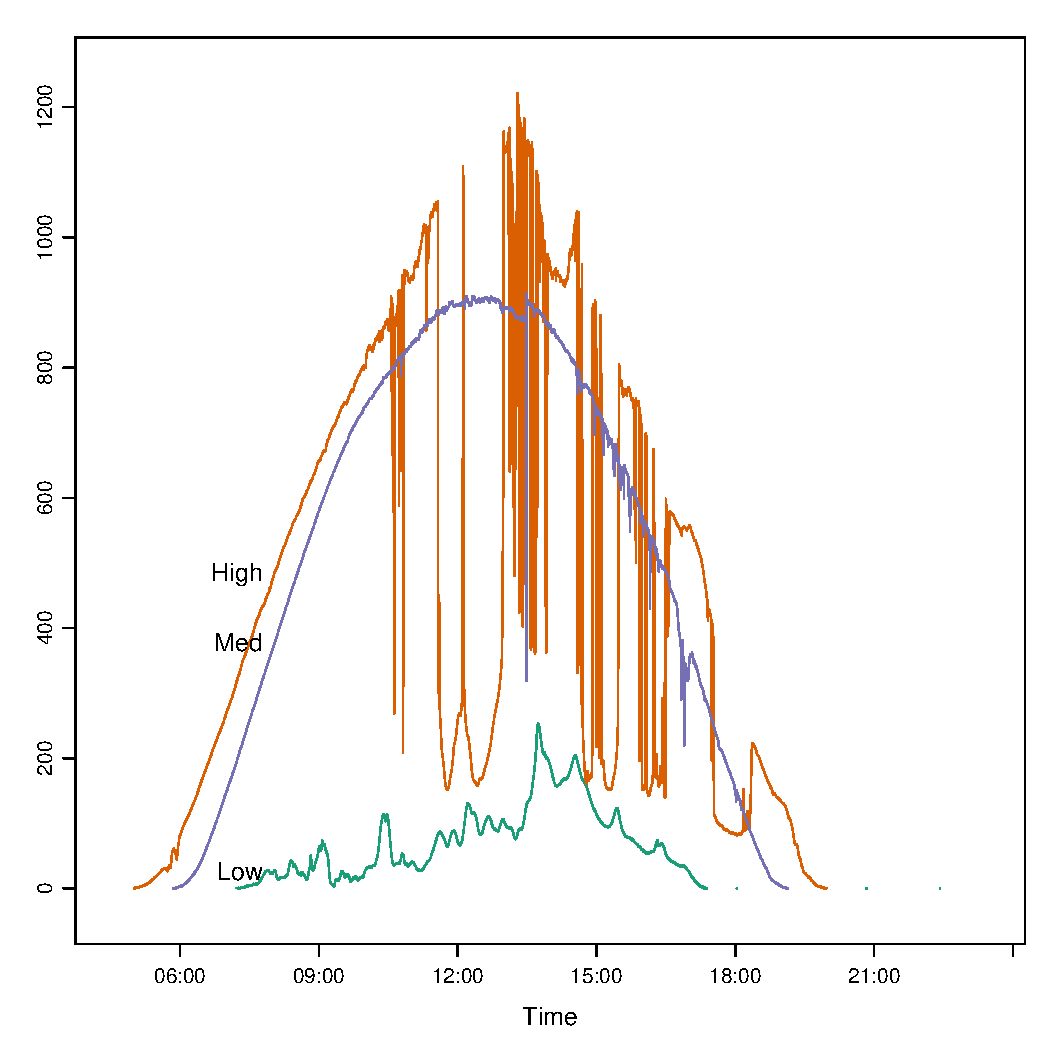
\includegraphics[height=0.75\textheight]{../figs/radLowMedHigh.pdf}
\end{center}
\end{itemize}
\end{frame}


\begin{frame}[label={sec:org20a79dd}]{Los Sistemas Fotovoltaicos y la Red Eléctrica}
\begin{itemize}
\item Los SFCR pueden proporcionar servicios de apoyo a la red gracias a
las funcionalidades que incorporan los inversores de conexión a red,
capaces de controlar la potencia activa inyectada en el punto de
conexión, y la potencia reactiva en funcionamiento normal o para
enfrentarse a huecos de tensión.

\begin{center}
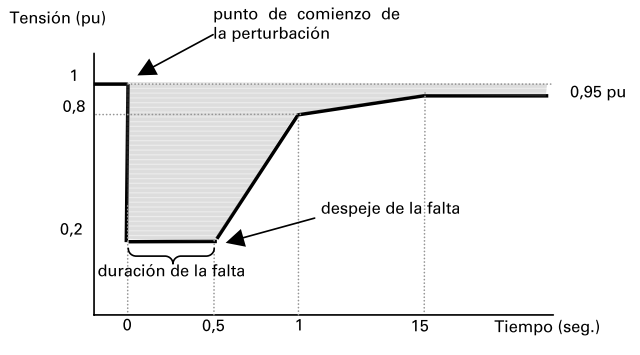
\includegraphics[height=0.7\textheight]{../figs/hueco-tension.png}
\end{center}
\end{itemize}
\end{frame}

\begin{frame}[label={sec:org041cefe}]{Variabilidad de la Radiación}
\begin{itemize}
\item La irradiancia solar es un proceso con inercia y con baja
probabilidad para mostrar cambios abruptos.

\item La probabilidad de ocurrencia de fluctuaciones elevadas es
sustancialmente menor al observar con resoluciones temporales
altas.
\end{itemize}

\begin{center}
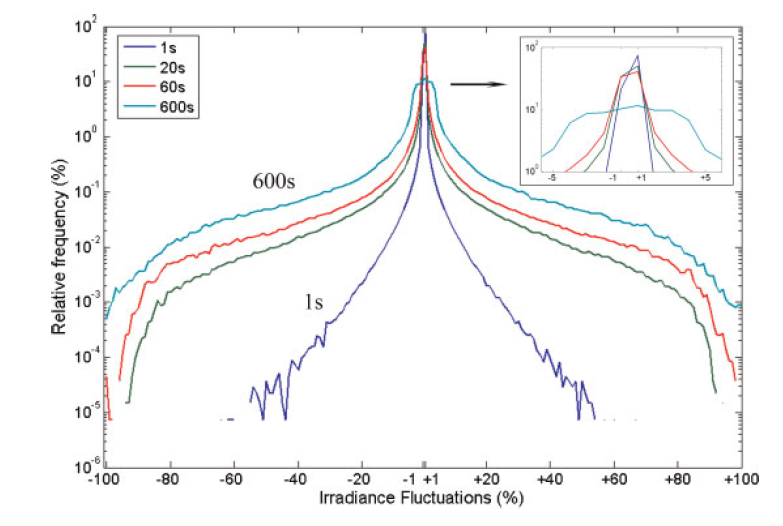
\includegraphics[height=0.65\textheight]{../figs/FluctuacionIrradiancia_Marcosetal2011.png}
\end{center}
\end{frame}

\begin{frame}[label={sec:org37be77f}]{Variabilidad de la Radiación}
\begin{itemize}
\item El nivel de fluctuación depende del comportamiento de la atmósfera (mayor en días parcialmente cubiertos).
\end{itemize}

\begin{center}
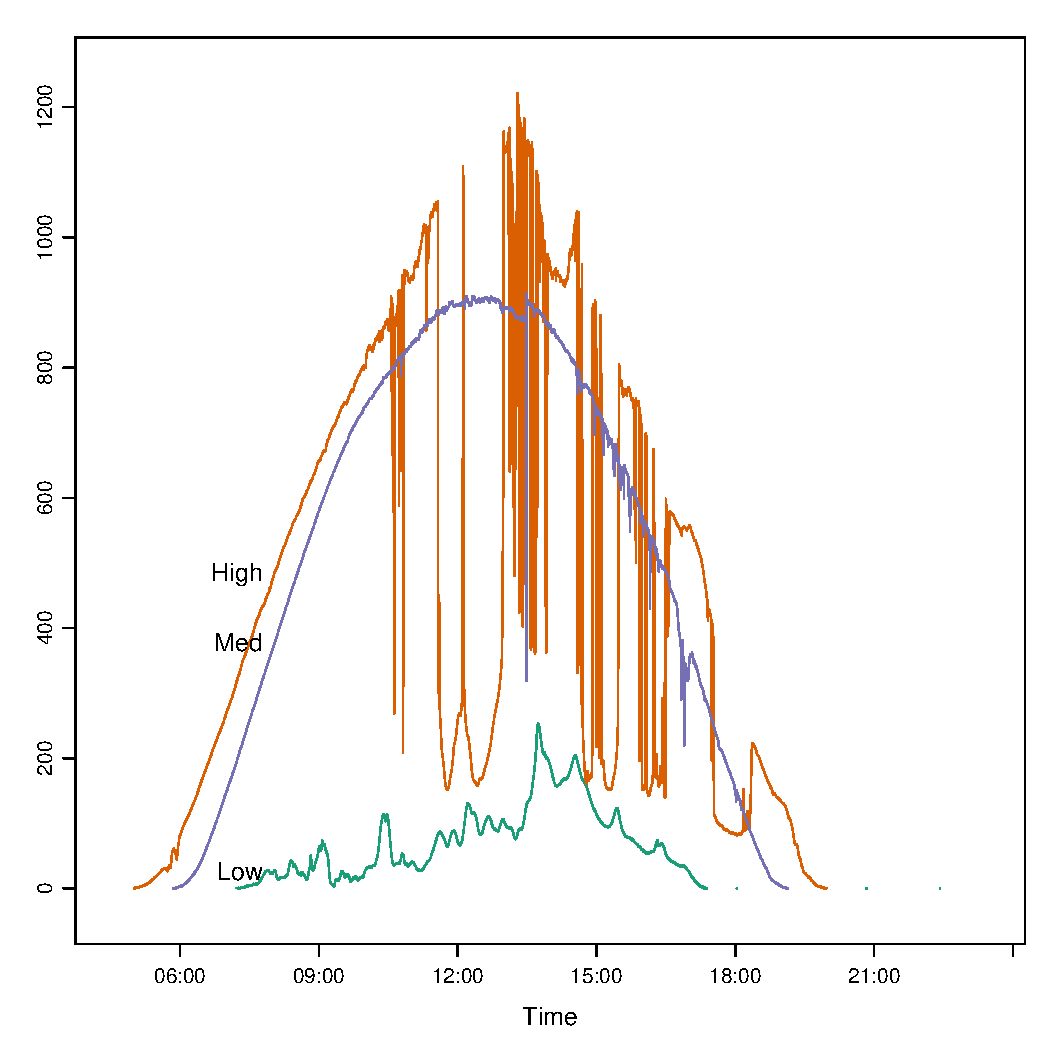
\includegraphics[height=0.65\textheight]{../figs/radLowMedHigh.pdf}
\end{center}
\end{frame}


\section{Incertidumbre y Predicción}
\label{sec:org1f108f3}
\begin{frame}[label={sec:org865d827}]{Potencia e Incertidumbre}
\begin{itemize}
\item La casación entre generación y demanda que se consigue en las redes
eléctricas se basa en la programación de las diferentes unidades de
generación disponibles para suministrar la demanda prevista y para
constituir reservas que hagan frente a las posibles variaciones en
la demanda.
\item Esta programación se produce en escalas y horizontes temporales
diversos y se actualiza de forma sistemática de acuerdo con las
variaciones previstas en la predicción de la demanda.
\item La inclusión masiva de sistemas fotovoltaicos en la red
modifica el equilibrio existente y puede implicar el uso de las
reservas de generación previstas originalmente para asumir las
variaciones de la demanda.
\end{itemize}
\end{frame}

\begin{frame}[label={sec:orgcee2165}]{Predicción de la Potencia}
\begin{itemize}
\item En este contexto el reto no es tanto la variabilidad como la
predicción de los cambios.
\item La realización de predicciones en horizontes horarios o diarios de
la potencia generada por un sistema fotovoltaico o por un grupo de
sistemas es crucial para facilitar la integración de sistemas
fotovoltaicos en redes eléctricas.
\item La predicción de radiación solar y potencia de sistemas
fotovoltaicos es un área de investigación de plena actualidad.
\end{itemize}
\end{frame}

\begin{frame}[label={sec:orgb020f25}]{Ejemplo: proyecto europeo PVCROPS}
\begin{itemize}
\item Herramienta de aprendizaje automático o \emph{machine learning}
entrenada con series históricas de predicciones NWP y medidas de
potencia eléctrica (30 días en la serie temporal de
entrenamiento).
\item Predicción de potencia AC con resolución horaria y un horizonte
temporal de 1 día.
\end{itemize}


\begin{center}
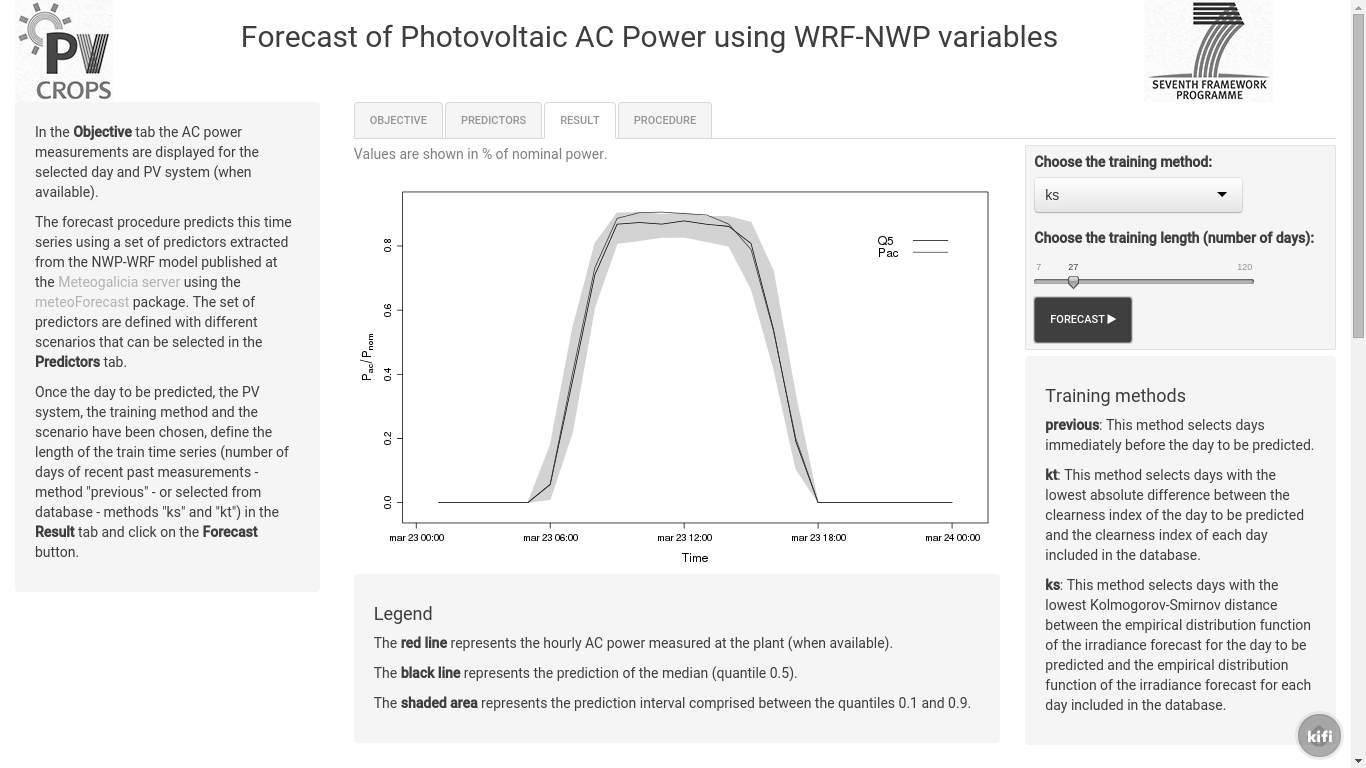
\includegraphics[height=0.5\textheight]{../figs/ForecastShiny.png}
\end{center}
\end{frame}

\begin{frame}[label={sec:org9034d88}]{Ejemplo: proyecto europeo PVCROPS}
\begin{itemize}
\item Se emplean como entradas las predicciones de variables
meteorológicas generadas por modelos de predicción meteorológica
numérica e índices de variación espacial y temporal estimados con
las variables meteorológicas.
\end{itemize}

\begin{center}
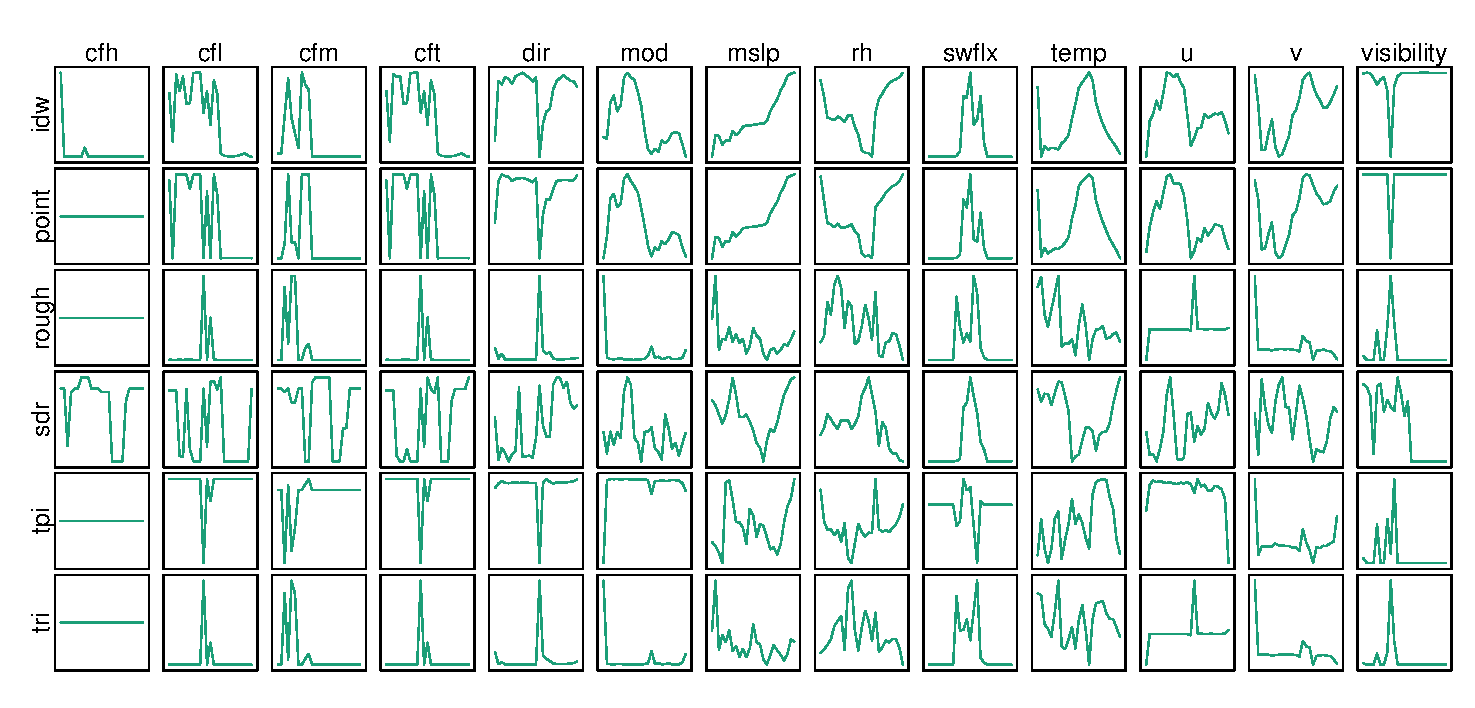
\includegraphics[height=0.7\textheight]{../figs/varsComplete.pdf}
\end{center}
\end{frame}


\begin{frame}[label={sec:orgfa175ba}]{Ejemplo: proyecto europeo PVCROPS}
\begin{itemize}
\item Genera predicciones probabilísticas, entregando tanto la mediana de
la predicción como un intervalo de confianza, que permite
cuantificar la fiabilidad de la predicción, y que puede servir como
medida indirecta de la variabilidad futura.
\end{itemize}

\begin{center}
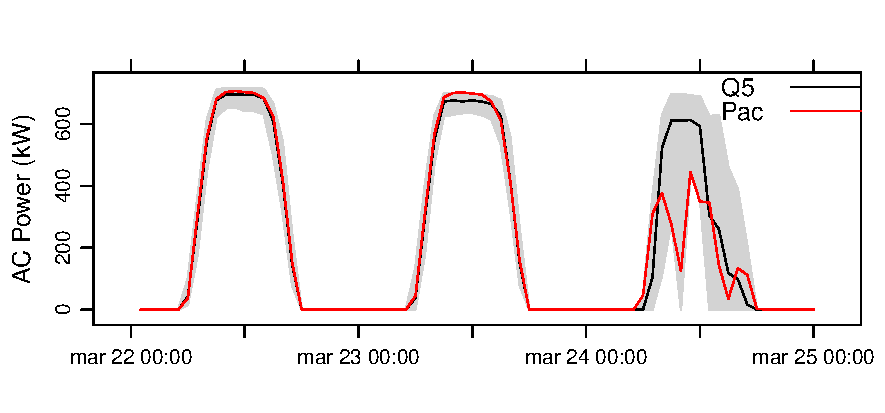
\includegraphics[width=0.6\textwidth]{../figs/powerResult.pdf}
\end{center}

\begin{center}
\url{http://vps156.cesvima.upm.es:3838/predictPac/}
\end{center}
\end{frame}


\begin{frame}[label={sec:org96e92a9}]{Predicciones agregadas}
\begin{itemize}
\item Las predicciones obtenidas mejoran cuando las predicciones se
aplican a un conjunto de sistemas.
\end{itemize}
\end{frame}

\section{Variabilidad de la Potencia}
\label{sec:org1aa2668}

\begin{frame}[label={sec:org1d85f84}]{Variabilidad de la Potencia}
El funcionamiento de la red eléctrica persigue el balance instantáneo
  entre la potencia generada y la potencia consumida, de forma que la
  variabilidad de los sistemas fotovoltaicos interconectados puede
  obligar al uso de otros recursos de la red que permitan restablecer
  el balance.
\end{frame}
\begin{frame}[label={sec:org9ea15e7}]{Variabilidad Conjunta}
La variabilidad presente en la irradiancia solar se atenúa:
\begin{itemize}
\item por la dispersión espacial entre diferentes centrales.
\item por la dispersión espacial dentro de una central.
\end{itemize}
\end{frame}
\begin{frame}[label={sec:orgbf3b009}]{Dispersión espacial entre centrales}
\begin{itemize}
\item En términos generales, la dispersión espacial de sistemas
fotovoltaicos diferentes conectados a la misma red atenúa la
variabilidad conjunta.

\begin{center}
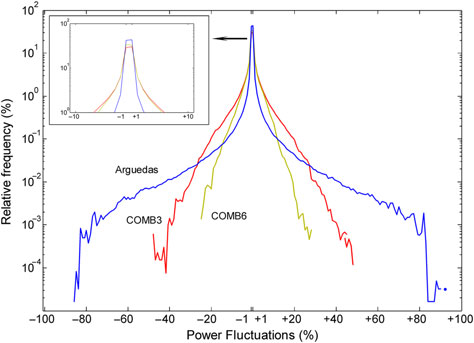
\includegraphics[height=0.5\textheight]{../figs/Variabilidad_DispersionGeografica_Plantas.png}
\end{center}

\item El nivel de atenuación depende principalmente de las
características meteorológicas de la zona y época, y de la
distancia entre los sistemas.

\item Para distancias mayores de \(\SI{5}{\kilo\meter}\) las fluctuaciones
de irradiancia con resolución temporal de 1 minuto están
esencialmente incorreladas.
\end{itemize}
\end{frame}

\begin{frame}[label={sec:orgf1a182b}]{Dispersión espacial dentro de una central}
En términos generales, la dispersión espacial de generadores
  fotovoltaicos pertenecientes a una misma central atenúa la
  variabilidad conjunta.

\begin{center}
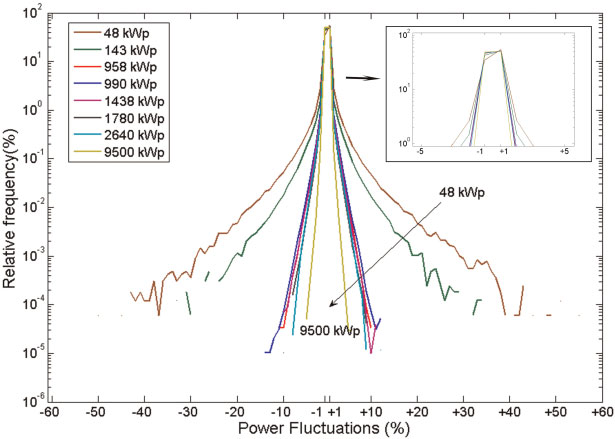
\includegraphics[height=0.7\textheight]{../figs/Variabilidad_DispersionGeografica_Planta.png}
\end{center}
\end{frame}

\begin{frame}[label={sec:orgdb9f711}]{Dispersión espacial dentro de una central}
\begin{itemize}
\item La correlación entre la potencia de cada inversor depende de la resolución temporal, la distancia entre los inversores, y el nivel de fluctuación del día en cuestión:
\begin{itemize}
\item Escalas temporales inferiores al minuto: correlaciones bajas.
\item Escalas temporales superiores a los 20 minutos: correlaciones altas y positivas que decrecen de forma exponencial con la distancia, y con una clara dependencia con el nivel de fluctuación diaria.
\item Escalas temporales intermedias: la correlación depende fuertemente del nivel de fluctuación diario.
\end{itemize}
\end{itemize}

\begin{center}
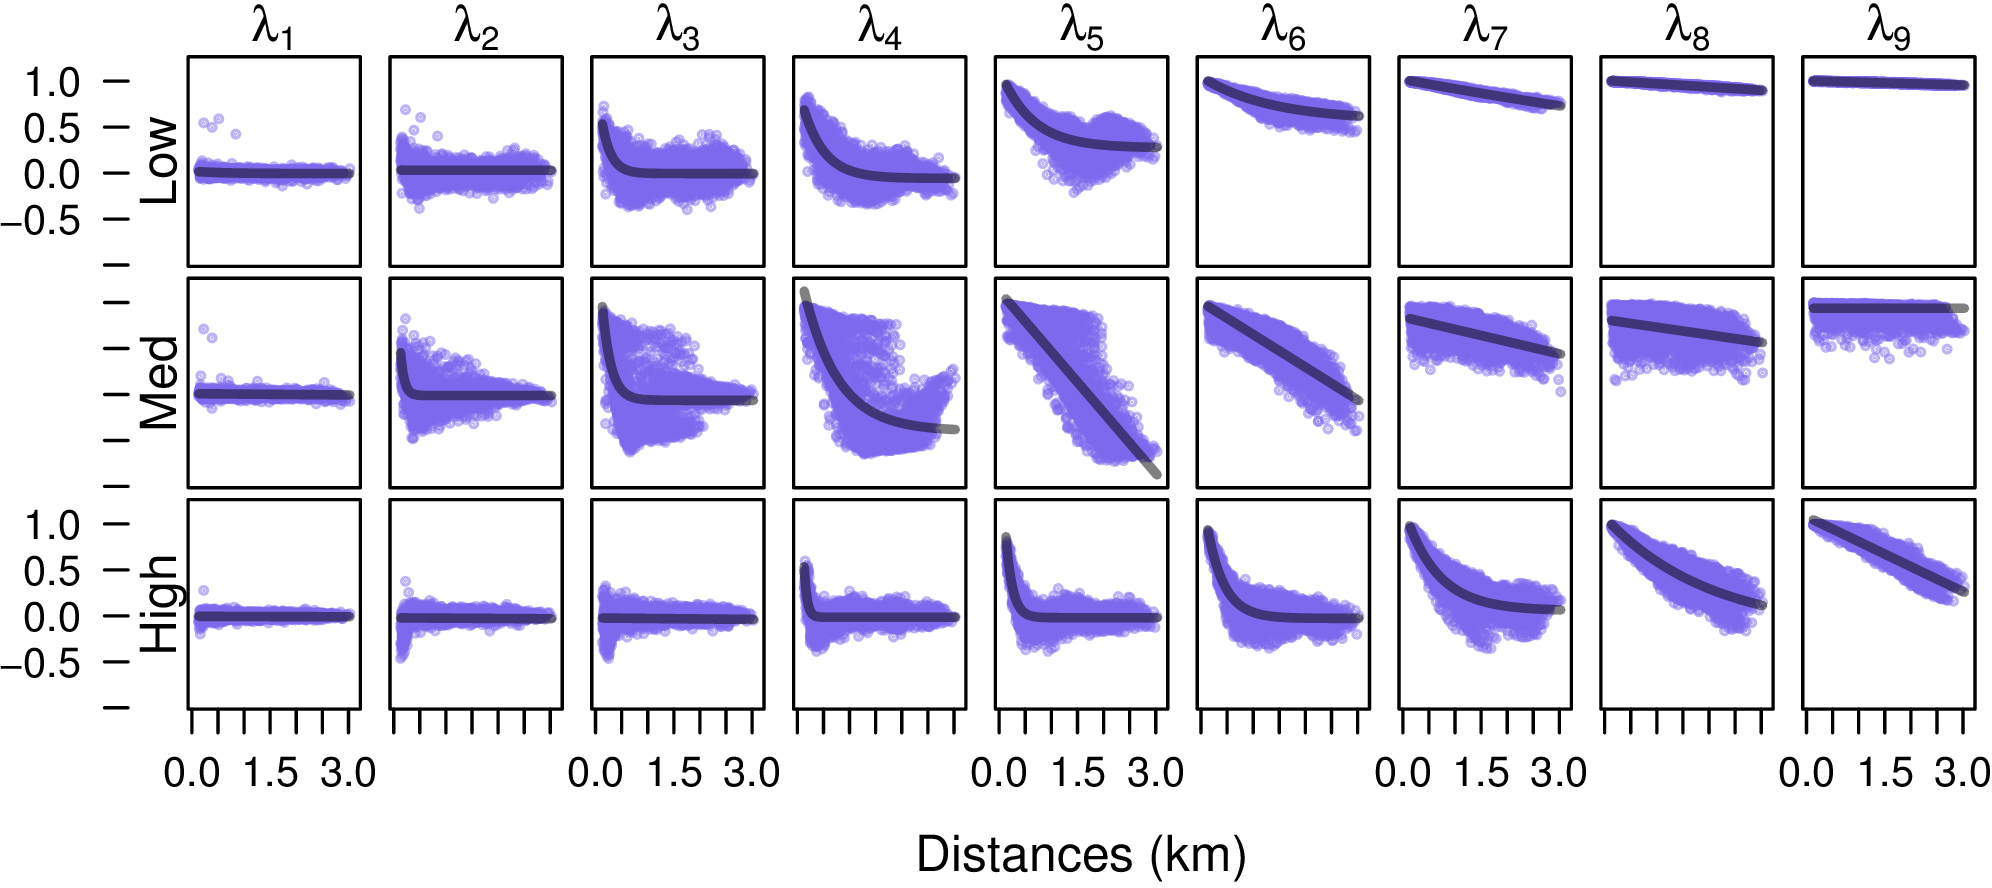
\includegraphics[height=0.6\textheight]{../figs/corDistMatrix_nls.png}
\end{center}
\end{frame}

\begin{frame}[label={sec:orga7d1a7d}]{Un sistema fotovoltaico es un filtro paso bajo}
\begin{itemize}
\item Las frecuencias altas son atenuadas porque no hay correlación
entre las diferentes series temporales,
\item Las frecuencias bajas permanecen sin alteración gracias a que la
correlación alcanza valores cercanos a la unidad
\item La atenuación de las frecuencias intermedias depende de la
distancia entre los inversores y el nivel de fluctuación diario
\end{itemize}

\begin{center}
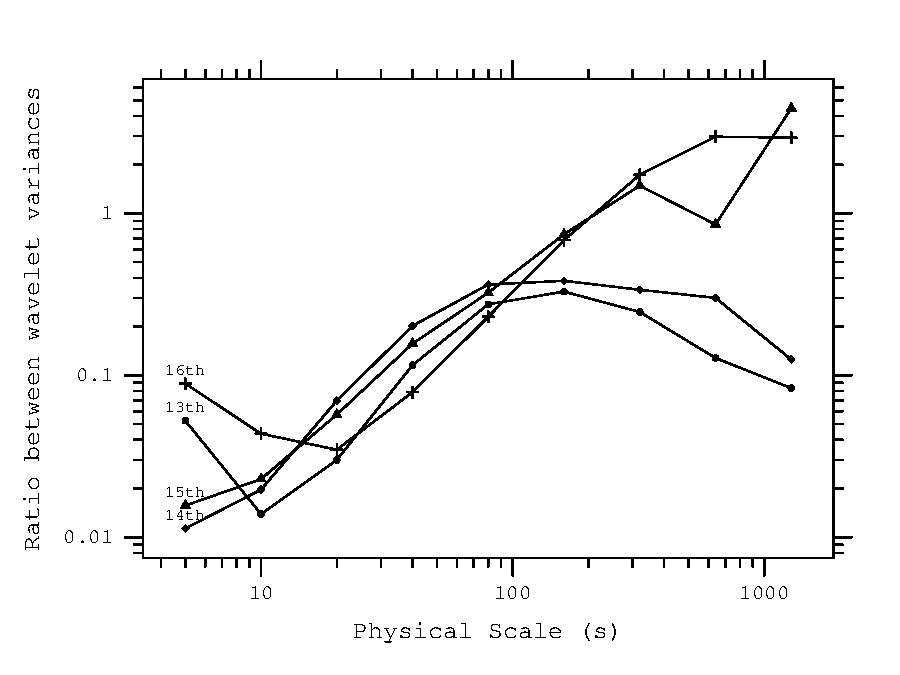
\includegraphics[height=0.55\textheight]{../figs/filtroPasoBajoWavelet.pdf}
\end{center}
\end{frame}

\begin{frame}[label={sec:orgc060118}]{Normativas de red}
\begin{itemize}
\item La variabilidad en escalas de tiempo bajas puede influir en mayor o
menor medida en el funcionamiento de la red eléctrica.
\item Existencia de normativas y recomendaciones para la integración de
sistemas fotovoltaicos en la red.
\item Ejemplo clásico: Autoridad Eléctrica de Puerto Rico incluye en su
normativa el concepto de rampa para cuantificar las fluctuaciones
admisibles:
\end{itemize}

\begin{quote}
A 10\% per minute rate (based on AC contracted capacity) limitation shall be enforced. This ramp rate limit applies both to the increase and decrease of power output and is independent of meteorological conditions.
\end{quote}
\end{frame}

\begin{frame}[label={sec:org1e086f4}]{Definiciones de rampas}
Uno de los problemas principales en este requerimiento (y otros similares) es que, aunque es fácil identificar visualmente una rampa en una serie temporal de potencia, no existe consenso en una definición formal que permita identificarla y cuantificarla.
\end{frame}

\begin{frame}[label={sec:org00907ab}]{Ejemplos de definiciones de rampas}
\begin{itemize}
\item Existe una rampa al inicio de un intervalo temporal si la magnitud del cambio en un instante temporal posterior es mayor que un umbral predeterminado.
\end{itemize}
\[ 
\left| P(t +\Delta_t) - P(t)\right| > \tau
\]

\begin{itemize}
\item Existe una rampa en un intervalo temporal si la diferencia entre los
valores máximo y mínimo supera un determinado umbral.
\end{itemize}
\[
\max(\{P_t: t = t_0, \dots, t_0+\Delta_t\}) - \min(\{P_t: t=t_0,
\dots, t_0+\Delta_t\}) > \tau
\]

\begin{itemize}
\item Existe una rampa dentro de un intervalo si el ratio entre el valor absoluto de la diferencia entre las medidas de potencia en dos instantes temporales, y la longitud del intervalo supera un determinado umbral.
\end{itemize}
\[
\frac{\left|P(t + \Delta_t) - P(t)\right|}{\Delta_t} > \tau
\]

\begin{itemize}
\item Existe una rampa en un intervalo si el valor absoluto de la señal de diferencias filtrada (por ejemplo, mediante una media móvil) supera un determinado umbral.
\end{itemize}
\end{frame}

\begin{frame}[label={sec:org8de00e7}]{Definición de rampas}
La elección de una métrica entre esta variedad de definiciones es un
\alert{compromiso} entre diferentes requisitos.

\begin{itemize}
\item Por un parte, la definición debe ser \alert{coherente y correcta desde un
punto de vista matemático}.
\item Por otra parte, los resultados que proporcione la métrica adoptada
deben ser \alert{útiles y dotados de significado}.
\item Finalmente, el concepto asociado a la métrica debe estar ligado a
las \alert{prácticas y requerimientos comúnmente empleados por los
operadores de la red}.
\end{itemize}
\end{frame}

\begin{frame}[label={sec:org144a388}]{Limitación de rampas}
La limitación de las rampas de los sistemas fotovoltaicos es un
requerimiento que se debe afrontar, principalmente en el caso de las
centrales fotovoltaicas de gran tamaño.

Existen tres estrategias principales:
\begin{itemize}
\item el uso de sistemas de acumulación energética;
\item acumulación energética combinada con predicción de rampas;
\item predicción de rampas sin acumulación.
\end{itemize}
\end{frame}

\begin{frame}[label={sec:org8512a43}]{Limitación de rampas}
\begin{itemize}
\item La inclusión de sistemas de acumulación, siendo la opción más
evidente en centrales de gran tamaño, conlleva aumentos en los
costes de instalación y en la complejidad y mantenimiento del
sistema.

\item Las herramientas de predicción de rampas combinadas con mecanismos
de control en el inversor fotovoltaico permiten reducir el tamaño de
la acumulación necesaria, e incluso se puede evitar su inclusión en
determinadas combinaciones de potencia instalada y requerimientos de
rampas admisibles.
\end{itemize}
\end{frame}
\begin{frame}[label={sec:orgdb06d63}]{Cálculo de sistema de acumulación}
\end{frame}
\end{document}